\chapter[SCP-118 核爆原生生物]{
    SCP-118 Nuclear Protists\\
    SCP-118 核爆原生生物
}

\label{chap:SCP-118}

\begin{figure}[H]
    \centering
    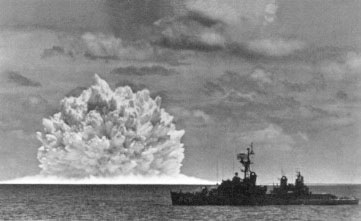
\includegraphics[width=0.5\linewidth]{images/SCP.118.jpg}
    \caption*{19██年█号红区收容失败时的照片}
\end{figure}

\bb{项目编号:}SCP-118

\bb{项目等级:}Euclid

\bb{特殊收容措施:}SCP-118的数量和分布状况导致不可能收容所有个体。已知的SCP-118“红区”(Red Zone)应以驻军或其它可信借口对所有平民海上船只和潜水员实行封闭。利用在SCP-118红区附近进行军事行动的海军中的人员关系使军用船只尽可能少穿过红区。若红区中任意区域深度不足1500米,则该限制同样适用于航空器。监控周边“黄区”(Yellow Zone)内一切人类活动,禁止任何接近红区的非军队船只和个人进入红区。在红区和黄区中应遵循协议“有毒的收成”(TOXIC HARVEST)以确保移除SCP-118制造的核弹。此外,应遵循协议“牢房监视”(CELL WATCH)以确保尽早发现成形中的红区。

SCP-118样品可通过无毒微生物SCP标准收容程序储存。

\bb{描述:}SCP-118是一种海洋原生生物,有能力利用海中的材料组装实用的自发性核弹。SCP-118尚属未知,因此科学界还未将其分类,不过其个体类似于裸藻门原生生物,但移动速度、营养储存能力和α辐射抗性都明显优于后者。SCP-118个体在全球海域均有发现。

处于适宜其生存的咸水环境中的SCP-118个体会搜集铁、银、铜、碳、TNT及铀同位素等材料。SCP-118找到所需材料后会将其吸收进细胞,方式视材料尺寸而定。单个原子和分子(大部分是溶解在水中的物质)通过专门的泵蛋白穿过细胞膜;大一些而比其细胞小的微粒通过吞噬作用被摄入;更大的材料会被不明机制分解为微粒,再被利用前两种方式吸收。该“采矿”过程甚至被应用于坚硬固体物质,如金属块。

吸收的材料量达到阈值后,SCP-118个体会来到所在水体底部的“组装区”组装核弹。被组装的核弹为使用铀-235作为裂变材料的枪式\footnote{译注:原子弹触发方式的一种。两块皆小于临界体积的半球形裂变物质分开一定距离放置,中子源置于两块裂变物质中间。核装药的球面上裹有一层反射中子的材料(提高链式反应效率),反射层外是高速炸药。起爆原子弹时,两块裂变物质在炸药的轰击下被迅速压缩为一个扁球,即刻达到超临界状态。中子源此时释放出大量中子参与链式反应,使裂变物质在极短的时间内释放出巨大的能量,最终使得原子弹爆炸。}裂变核弹。对组装过程中的核弹的观察表明,首先完成的是其圆柱形金属外壳,之后是两块亚临界铀和使铀互相结合的常规爆炸物。\dd{目前不清楚SCP-118如何浓缩收集到的铀。}(参见附录4)最后组装的是两块铀碰撞时所在的铀-238中子反射器,以及引爆器。SCP-118似乎是通过向(最初)微小的材料“种子”上添加微量材料来组装必要组件的。不同类的原子和分子可用于同一组件,做好的组件也不一定相同。尚不清楚SCP-118是以原子还是以亚微米级碎片为单位向种子添加材料的。SCP-118将材料和种子无缝接合的方法不明。组装所需时间取决于核弹大小、水体环境和矿物可用度,但观测显示制造一颗中等大小的核弹平均需要300天。

完成一颗核弹后,SCP-118就会做好其引爆器中的电路,使其爆炸。记录到的由SCP-118引发的核爆炸中约90\%的当量在20到35千吨之间,但也有低至4千吨和高达███千吨当量的报告。除人为干预的事例外,从未观测到引爆失败:所有记录在案的核弹或是被自行引爆,或是在完成之前就被打捞出水。SCP-118制造的核弹比设计和当量相似的人造核弹大,可能是因为在制造过程的大部分时间里将铀隔开的水的中子慢化效应。一个组装区在任意时刻一般都有1到3颗组装中的核弹,但也曾一次观测到多达6颗核弹。在同时组装多颗核弹的区域中,各核弹之间存在足够的距离,以防止其中一颗爆炸后摧毁或引爆其余核弹。

虽然基金会无法阻止平民和其他机构获得SCP-118样品,但其表面上与其它已知种类相似,数量稀少(相对于所有海洋原生生物而言),在材料丰富的水体之外没有异常表现,基金会也对可能发现异常生物品种的科学研究进行了标准监控。以上几点确保了通过细胞样品发现SCP-118真正性质的可能性极小。

基金会目前知道6处运作中的SCP-118组装区。虽然曾观测到一个组装区自然消失,但SCP-118的研究员目前的共识是无法在不造成大规模显著影响的情况下消除组装区(详情参见实验记录118-Gamma)。因此,应在SCP-118的组装区(命名为“红区”)和外围的“黄区”建立起收容。此外,应监控SCP-118数量偏高的区域(“关注区”,Zone of Interest)中组装区的迹象。

\tred{+ 收容区域列表——需要4级权限:}

\tred{- SCP-118收容区域}

\bb{红区(RZ):}

RZ - 1\\
位置:中大西洋\\
坐标:{[}编辑]\\
区域指挥官:Romanov上校\\
注:USS ████████\footnote{译注:USS为“United States Ship”的缩写,直译为“美国船舰”,专指美国海军的现役船舰。黑条部分为该船舰名称。}事故发生在距此红区██公里处。

RZ - 2\\
位置:北太平洋\\
坐标:{[}编辑]\\
区域指挥官:Chambers上校

RZ - 4\\
位置:南太平洋\\
坐标:{[}编辑]\\
区域指挥官:Knapp上校

RZ - 5\\
位置:印度洋\\
坐标:{[}编辑]\\
区域指挥官:Wayne上校\\
注:邻近航道,核爆容忍度低

RZ - 6\\
位置:北大西洋\\
坐标:{[}编辑]\\
区域指挥官:Fazil上校\\
注:邻近美国SOSUS\footnote{译注:“SOund SUrveillance System”的缩写,意为“声音监听系统”,是美国在冷战期间设置的一套用于监测深海的系统,沿用至今。}水听器\footnote{译注:把水下声信号转换为本质上等效的电信号的仪器。},核爆容忍度低

RZ - 7\\
位置:{[}编辑]\\
坐标:{[}编辑]\\
区域指挥官:████████上校\\
注:红区位于████████市境内。同时,该红区的平均深度较浅,所在地区航运繁忙,加上██████和██████间局势持续紧张,且市内有一座核电站,另有基金会人员和设施,因此不能允许该红区发生核爆炸。此外,地区内繁忙的航运和城市上空的大量空中交通使得任何长期的准入限制均不现实。

\bb{关注区(ZOI)}

ZOI - 1(北纬█████,东经█████)——SCP-118数量每年提升5\%左右,ZOI面积每年约增长3\%。\\
ZOI - 3(北纬█████,西经█████)——ZOI内有约20口油井,SCP-118数量和ZOI尺寸暂时稳定。

\bb{历史区域(Former Zone,FZ)}

FZ-RED-3(北纬█████,东经█████)——前RZ - 3,最后一颗核弹组装于1992年,SCP-118数量于20██年降至海中平均值。\\
FZ-ZOI-2(北纬█████,西经█████)——前ZOI - 2,SCP-118数量于1986年降至海中平均值。

\bb{附录-118-1:}USS ████████事故之后,增加了划定红区时使用的禁区半径。更新收容协议“有毒的收成”。

\bb{附录-118-2:}《部分禁止核试验条约》出台后,随着越来越多更加有效的核爆炸探测方法被投入使用,SCP-118核爆造成的负面后果有所增加。根据以上事实修订了收容协议。

\bb{附录-118-3:}由于收容SCP-118红区的开销巨大,O-5议会要求试验可能清除SCP-118组装区的方法。

\tred{+ 实验记录118-GAMMA——需要4级权限:}

\tred{- 红区根除试验——总结}

\begin{scpbox}

\bb{引言:}能读到SCP-118档案的研究员可以提交附带损害\footnote{译注:collateral damage,军事行动中对无关平民及民用建筑的损害。}在可接受范围内的根除SCP-118组装区的提案。O5议会通过的提案将被执行。试验在█号红区进行。

\bb{提案:}使用紫外线发射器对未完成的核弹及邻近区域进行杀菌。\\
\bb{O5意见:}通过\\
\bb{结果:}未完成的弹头周边区域一开始没有微生物,但SCP-118数量在一小时内回到普通水平。\\
看来对区域的非持续性杀菌达不到目的。我们想到的任何方法都必须让红区,或者至少红区的海底在较长的一段时间里不含SCP-118。——Brant博士

\bb{提案:}向海底灌次氯酸钠。\\
\bb{O5意见:}否决\\
\bb{结果:}N\slash A\\
哪个蠢蛋说往海里倒漂白剂的?这些化学品在起效之前漂得也太远了。足以减小SCP-118数目的量会对生态造成极其严重的破坏。——Klaus博士

\bb{提案:}对海底进行深水炸弹地毯式轰炸以破坏组装中的核弹。\\
\bb{O5意见:}否决\\
\bb{结果:}N\slash A\\
一方面这样会超出我们的海军预算,另一方面引爆核弹内的常规爆炸物导致核弹提前起爆的概率太高了。这也会让我们的行动更容易被水听器监测到。——Klaus博士

\bb{提案:}用钴-60定向伽马射线发射器“清扫”海域。\\
\bb{O5意见:}通过\\
\bb{结果:}尽管该方法让被“清扫”的区域无菌,但其速度太慢,远远不能在个体返回区域前清理完整片红区。保持整个红区无菌需要的发射器和船只数量完全不现实。\\
虽然发射器没办法为我们除掉红区这事挺可惜的,但我觉得可以把它给我们的核弹回收队用。伽马射线可以给我们回收的核弹灭菌,预防差不多完成的核弹在回收的时候爆炸。伽马射线还能照到我们现有的化学品和紫外线灭菌法无能为力的区域。——Thomson上校(RZ - 3区域指挥官)

\bb{提案:}用塑料膜遮罩红区的海底。\\
\bb{O5意见:}批准在一枚组装中的弹头上进行概念验证\footnote{译注:proof of concept,对某些想法的一个较短而不完整的实现,以证明其可行性,示范其原理,其目的是验证一些概念或理论。}。\\
\bb{结果:}首次尝试未能成功在弹头周围实现防水密封。第二次尝试时膜在海洋环境中太不牢固,被从固定点扯下。第三张膜更厚,更结实,但于数小时内出现了几百个微小的破洞,这可能是SCP-118的“采矿”行为所致。\\
考虑到已知SCP-118能够蚀穿旧炮弹来收集内部的爆炸物,这没啥好吃惊的。我们指望过拿掉组装区会比拿掉原材料更有效。——Klaus博士

\bb{提案:}向海底输送██████化合物。\\
\bb{注:}由现工作于██号生物研究站点化学研究部门的前SCP-118研究员██████████博士提出。测试证实此种化合物对SCP-118而言是致命的,且集中在水底,在水中可于15小时内降解为较为无害的物质。\\
\bb{O5意见:}通过\\
\bb{结果:}一周内,SCP-118在海底的数量降至原数量的3\%。未观测到红区内的两颗已知的未完成核弹有进展迹象。然而,实验开始230天后,红区以北60km处探测到一次核爆。对该区域的测量显示SCP-118数量大大增加,爆炸点周边区域因此被重归类为红区。此外,某些海洋细菌出乎意料地分解了██████化合物,产生的有毒副产品造成被处理区域中的鱼类大量死亡。停止实验后观测到红区慢慢“转移”回原地点。\\
看来让红区不可用只是让SCP-118的组装区移到了一个新地点。尽管如此,也许如果我们能够改良██████化合物或者找到一种应用起来更不容易察觉的新化合物的话,我们就可以把红区移到离人类居住区或者商业活动区远的地方。——██████████博士

\bb{提案:}使用SCP-████。\\
\bb{O5意见:}通过\\
\bb{结果:}{[}数据删除]\\
\bb{注:}SCP-████被重分级为Euclid。——Klaus博士

\bb{结论:}由于使用██████化合物和SCP-████造成的后果,媒体对█号红区周边区域的关注度上升了。加上提案均带有引发严重附带损害的高风险,在█号红区的测试被暂停。

\end{scpbox}

\bb{附录-118-4(需要4级权限):}

\begin{scpbox}

我们的研究已经发现SCP-118利用铀-235稍稍比铀-238更容易变成高氧化态的事实来浓缩铀。已收集到大量铀且靠近组装区的SCP-118个体会生出专门的细胞器,那是一系列的数千个类似于液泡的腔,内含与线粒体相似的细胞器,负责催化还原和氧化反应。在一个腔中,铀被不停地还原和氧化。氧化态高的铀化合物被运往腔组成的“链”上部,氧化态低的化合物被运往下部。最终在链的一端可得到少量高浓缩铀。

█号研究部门的研究员和工程师已经设法做出了一个以SCP-118运用的原理为基础的铀浓缩设备原型机。虽然原型机要花费长得过分的时间才能制造武器等级的铀,但它成功造出了反应堆等级的铀,尽管成本远大于常规方式。虽然目前有种种限制,不过这个想法挺有希望,我已经把我们的研究结果送到相关的掩护公司\footnote{译注:front company,由另一个组织设立并控制的公司,可代替其上级组织实施行动,而不使这些行动与其上级组织联系起来。}了。

——████████博士

\end{scpbox}
